\chapter{Design}
\label{chapter:design}

{\project} is composed of two parts:
\begin{enumerate}
  \item A backend that communicates with the Twitter API, retrieves tweets that match the query provided by the user, performs parsing and clustering. The result is a list of messages annotated with the cluster id they belong to. This information is made available with the help of an HTTP server that exposes an API. We have chosen JSON as the format to export the data via the API.
  \item A frontend that takes the JSON and renders clusters of tweets as well as provides an interface for the user to explore the conversations 
\end{enumerate}

\begin{figure}[ht!]
\centering
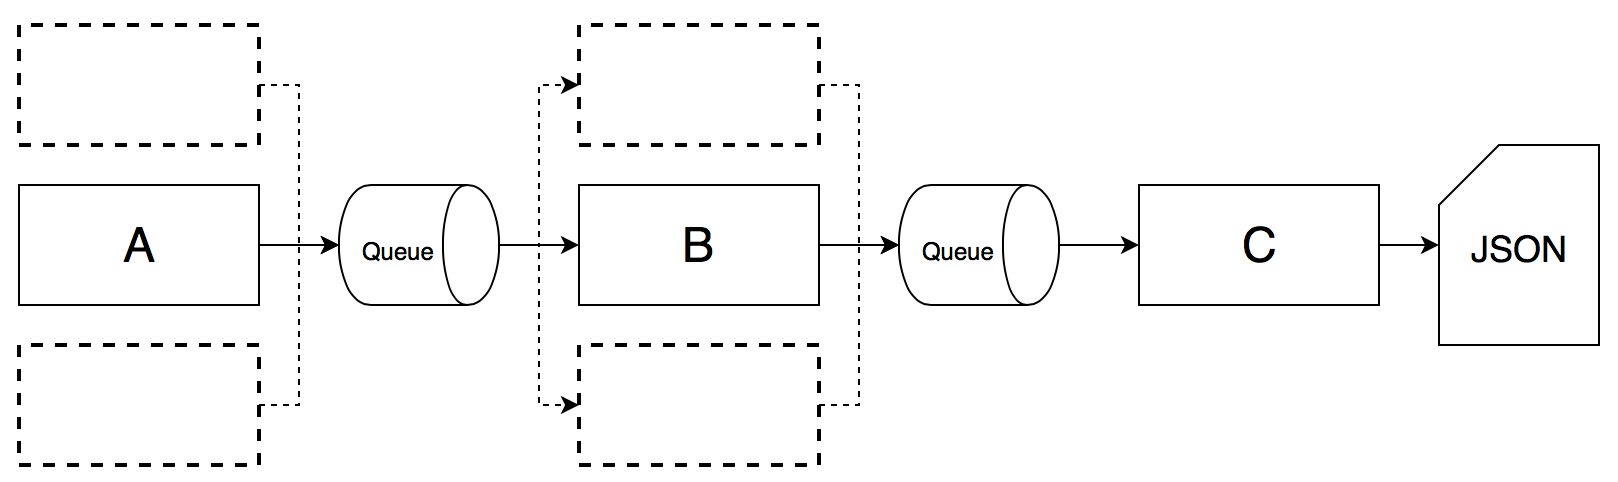
\includegraphics[width=\textwidth,height=\textheight,keepaspectratio]{src/img/design.png}
\caption{Design for the data processing pipeline\label{overflow}}
\end{figure}

The data processing pipeline is composed of three main parts. Data acquisition (marked with A in the design) is responsible for fetching data that will later be processed, the component is agnostic of the data that passes through but in our case it is Twitter messages (tweets). It uses a library \footnote{http://twitter4j.org/en/index.html} to communicate with Twitter API, it retrieves the tweets and stores them in a queue. The queue library is provided by Apache Kafka \footnote{http://kafka.apache.org}. As shown in the design, the reason for using queues between intermediary steps is that they allow for the producer and consumer to operate and different frequencies. The data acquisition segment could launch several clients regardless of what is happening further down the pipeline.

The second section (B), data processing, parses the raw tweets and converts them into shorter messages with key terms. Messages are read from the queue that is being filled by the data acquisition layer (A). The processed messages are written to a new queue, thus allowing this layer to scale just as the previous one. Tweets are parsed and using StanfordNLP library \footnote{http://nlp.stanford.edu/software/index.shtml} each word is categorized with its own part-of-speech tag. Tags such as personal pronouns, possessive pronouns, prepositions, conjunctions are removed because they are too common. We could easily spin up several clients that consume messages because reading and writing is performed using two queues and thus the layer is decoupled from the other components of the pipeline. One issue related to parsing conversations especially ones from social media is the jargon used and possible spelling errors. This issue is exacerbated by the fact that Twitter conversations have such hard limits on the number of characters, on overage a message does not have more that 10-12 words.

The last part that processes data is responsible for clustering the messages based on the keywords generated in the previous step. The clustering algorithm uses K-Means with cosine similarity as a distance function, which I will go into more detail in the following section.

The visualization ({\frontend})  is rendered in the browser. This offers the advantage of being able to explore the profile of Twitter users and see the messages and their context. It works by polling the webserver that is serving a JSON file through it API. When new data becomes available it renders the clusters and the corresponding adjacent nodes. The polling process will continue in the background. From the user interface you are able to see the clusters and quickly identify large clusters. You are able to see all the clusters that belong to it either by hovering over the nodes or clicking the cluster and getting an expanded view with all messages.

\section{Implementation}
\label{sec:implementation}

In the following paragraphs I will go into further details on how the system is implemented.
\newline
The implementation is done in Scala\footnote{http://www.scala-lang.org}. The reason behind this choice is the fact that Scala enables us to use a functional programming paradigm and at the same time provides a type system that makes implementation easier. Many of the operations in the application include transformations of lists of messages, something that functional programming is very good at. At the same time the Scala source code is intended to be compiled into Java bytecode and run on the JVM. This allows us to include any Java library into the project as Scala was designed with Java interoperability in mind.
\newline
Another benefit of Scala is their implementation of parallel processing into the standard library. The aim of the language designers was achieving a high level abstraction that is easy to use thus achieving efficient parallel computations over collections in a transparent manner.
\begin{lstlisting}[caption=Example of parallel collection usage in Scala, label=scala_parallel_collections]
// Example of using parallel collections in Scala

list.map(_ + 42) // regular, sequential map over a collection
list.par.map(_ + 42) // parallel processing of the collection
\end{lstlisting}
Using a similar approach we can speed up message parsing and also the clustering step. This decision has had beneficial results for the overall processing time of the Twitter messages. We will go into further details about the running time and speed benefits of parallel processing in the pipeline in the Testing and Evaluation section.
\newline
\newline
Accessing the Twitter API requires a developer account and an application created on their website dev.twitter.com \footnote{https://dev.twitter.com/streaming/overview}. The application gives you access to public, user or site streams. We will be using the public streams which returns data flowing through Twitter in real time given a certain array of keywords. This is the most useful endpoint for our data mining usecase.Using the provided API authentication tokens you can configure twitter4j library to retrieve tweets that match a specific keyword (or multiple keywords). The library comes with OAuth support and handles authentication with the endpoint. All messages received are passed to queue.
\newline
\begin{figure}[ht!]
\centering
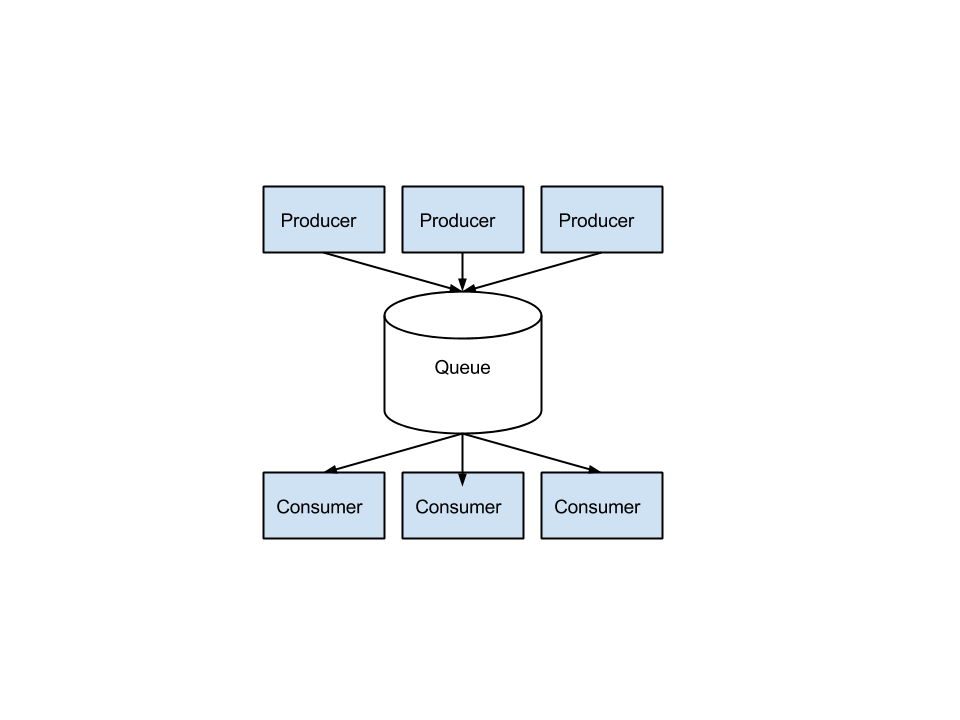
\includegraphics[width=\textwidth,height=\textheight,keepaspectratio]{src/img/queue.png}
\caption{Design for queue processing in the pipeline\label{overflow}}
\end{figure}
\newline
The messages retrieved are stored in a queue provided by Apache Kafka\footnote{http://kafka.apache.org/documentation.html\#introduction}. The queue, has a configurable storage period for the messages which allows us to use it for temporary storage.  Communication between producers, consumers and the queue is done via a binary protocol over TCP so message delivery is always assured. The protocol does not require a handshake step in order to get or put messages in the queue, after a socket connection is established the client simply writes the messages it requires as request and then reads them. Kafka also guarantees message order and load balancing over a group of consumers but these features are not of interest for our project. Using a queue provides an advantage over the fact that messages arrive and are consumed at different frequencies. Depending on the popularity of the keywords specified tweets can come in at different rates. Based on a series of tests the rate of messages has been up to 150 per minute. At the same time the StanfordNLP has a parsing speed of one tweet per second. Using a queue also means that it is possible to start several consumers and producers at the same time. A consumer is concerned with getting the messages out of the Apache Kafka queue and placing them in a a new queue where they will eventually be parsed. The Apache Kafka documentation lists "Stream Processing" as an ideal use case for the library, and the processing of the Twitter API feed is exactly this sort of use case, thus confirming our design decision.
\newline
Before applying the clustering algorithm the tweets are first parsed. Parsing the tweets means removing all non alphanumerical characters or punctuation: such as unicode characters. One of the reasons for removing non-alphanumerical characters is that the StanfordNLP library cannot parse emojis \footnote{An emoji is a pictogram, similar to ASCII emoticons, which have been incorporated into Unicode meaning a wide adoption in online communication. Emoji symbols are two-byte sequences and support for them in browsers and mobile devices varies.}.
\newline
The new messages are annotated using StanfordNLP part-of-speech tagger library. This library reads the text and assigns a part of speech or other token to each word. The set of part of speech tags follows the Penn Treebank Project \footnote{https://www.ling.upenn.edu/courses/Fall_2003/ling001/penn_treebank_pos.html}. The resulting output is a list of tuples containing of the word, its POS tag and its level in the dependency graph. The dependency tree is constructed by drawing an edge between a token and the all others that it determines. The tagger has an accuracy of 97.24% accuracy. More information about the implementation details and ideas that went into the project can be found in the paper \textbf{Feature-Rich Part-of-Speech Tagging with a Cyclic Dependency Network} by Kristina Toutanova, Dan Klein, Christopher Manning, and Yoram Singer.
\newline
The next step is to filter out words based on the part-of-speech tagging. Tags such as personal pronouns, possessive pronouns, prepositions, conjunctions are removed because they are too common and might introduce false positives for the clustering algorithm.
\newline
These parsed messages are pushed to a new queue. The reason for this is to completely decouple the 3 different stages of the pipeline: 
\begin{enumerate}
	\item Retrieving messages in realtime from Twitter using its API.
	\item Tagging the messages with their part-of-speech tag and using this to filter out common terms.
	\item Running the clustering algorithm using the parsed messages as input.
\end{enumerate}


The final stage of the pipeline takes all the parsed messages from the queue and applies the clustering algorithm. The algorithm used for this step is K-Means clustering and the distance function is the cosine similarity. Because the design of the K-Means clustering algorithm is to start the iterations with a random seed consisting of randomly selected points (in our case messages), we run the clustering using different starting seeds and choose the highest value out of all the runs as our best clustering option. This in turn will affect the overall running time of the application as we will see. Depending on our goals either speed or precision we can choose to just rely on the first random seed provided.
The name K-Means, first introduced in \textbf{Some methods for classification and analysis of multivariate observations} by J. MacQueen. K-Means is an important clustering algorithm; its objective is to minimize the average distance between a point and its cluster center where a cluster center is the mean of all points in that cluster.

\subsection{Clustering Algorithm}
\label{clusteringalgorithm}

The first step of the algorithm is to compute the TF \abbrev{TF}{Term frequency} (term frequency) and IDF \abbrev{IDF}{Inverse document frequency} (inverse document frequency) for each of the tweets. TF-IDF is a numerical statistic intended to provide information about the importance of a word in a document. TF is a direct measure for the number of times a word appears in a document while IDF helps scale down that measure for words that tend to appear often and scale up for words that are rare.

\begin{equation}
	\text{TF(D, t)} = {\sum \textrm{occurrences of t in D} \over
						\sum \textrm{number of terms in D}}
\end{equation}

The TF of a term \textit{t} in a document \textit{D} is the total number of occurrences of that term divided by the total number of terms in the document. A document in this case would constitute a tweet. And the terms we are computing TF for are all the terms that remain after the filtering in the previous stage.

\begin{equation}
	\text{IDF(D, t)} = { \log \bigg( {\sum \textrm{total number of terms in D} \over
						\sum \textrm{total number of occurrences of t}} \bigg) }	
\end{equation}

The IDF of a term \textit{t} in a document \textit{D} is the total number of terms in \textit{D} divided by the total number of occurrences of \textit{t} in \textit{D}. The document in this case constitutes all of the available tweets that we are attempting to cluster. The number of occurrences is also computed taking into account all the available messages.
\newline
Using TF and IDF we transform each tweet into a vector with weights for each of the terms. This way we can use the cosine similarity as a distance function in the clustering algorithm. Cosine similarity is a way of computing the similarity of two vectors by measuring the cosine of the angle between them. The cosine function output is in the range [-1, 1] where -1 means that the vectors have opposite directions and 1 means that they have the same direction. 

\begin{equation}
	\text{cosine similarity(A, B)} = {\sum_{i=1}^{n} A_i \times B_i \over
				\sqrt{\sum_{i=1}^{n} A_i^2} \times \sqrt{\sum_{i=1}^{n} B_i^2 }}
\end{equation}
\newline
The \textit{A} and \textit{B} vectors in our equation constitute two vectors i.e. two tweets that have been turned into vectors after computing their TF and IDF. And the result of the \textit{cosine similarity} function tells us how similar the two vectors are, in return how similar two tweets are.
\newline
\newline
The clustering algorithm uses the K-Means clustering algorithm.
To define some terms that are used in the implementation of the algorithm, a cluster center is the mean of all points in that cluster, or more formally

\begin{equation}
\text{ $\mu$ (w)} = { {1 \over |w| } {\sum_{x \in w} \textrm{ x } } }	
\end{equation}


Where \textit{w} is the cluster. Ideally the clusters that are formed do not overlap. To get a sense of how well a centroid, the mean point of a cluster, represents all of its members, we define RSS \textit{residual sum of squares}

\begin{equation}
\text{ RSS } = {{\sum_{x \in w_{k}}} \textrm{ | x - $\mu$(w)|$^{2}$ } }
\end{equation}

The objective of the algorithm, and therefor our objective is minimizing this RSS function. By reducing this value we reduce the average squared distance which is a measure of how well points in a cluster are represented by their centroid.

The algorithm starts with an initial set of clusters chosen at random from all the tweets. It then uses the distance function (the cosine similarity described above) to assign the rest of the tweets to those clusters. For each cluster now formed it computes a weighted average. These steps are repeated only now we use the weighted average centroids instead of the random points until the centroids remain the same between 2 consecutive steps or until an upper bound of steps is reached. This upper bound is added in to ensure the algorithm halts if it fails to reach convergence in a fixed number of steps.
\newline
There are a number of termination conditions we can apply:
\begin{enumerate}
	\item Terminate when RSS falls below a certain $\epsilon$
	\item Centroids do not change between iterations
	\item Assignments of points to clusters do not change over iterations
	\item A fixed number of iterations has completed. This will always ensure the termination of our algorithm but it might also affect the quality of our results.
\end{enumerate}
Several issues we might run into while running the algorithm are data outliers. An outlier is a data point on a graph or in a set of results that is very much bigger or smaller than the next nearest data point. Therefor such points do not fit well in any cluster being to far away from the rest of the data. One such example would be having a cluster with only one message.
\newline 
\begin{figure}[ht!]
\centering
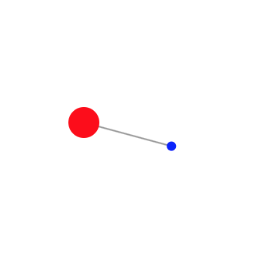
\includegraphics[resolution=300,keepaspectratio]{src/img/outlier.png}
\caption{Example of cluster rendering with outlier\label{overflow}}
\end{figure}
\newline
Another such example of clustering done sub optimally is having a cluster with no actual messages in it. This is due to the methods used to select the initial seeds for the clustering algorithm. Selecting a "bad" seed, by which we mean an outlier will always lead to sub optimal results. Heuristics used to improve results are using the RSS function to choose the seeds. By using this method we would go through different seed candidates and chose one. Another possible method is simply removing outliers from our sample data.
\newline
Different assignments yield different clusters which in turn have different weights. A higher weight means better similarity between the node and the cluster they belong to and therefore a better result. This similarity is computed with the help of the \textit{cosine similarity} function after the K-Means algorithm has finished its assignment. For better results several iterations of the algorithm are used and the best score is chosen, at the cost of time spent clustering.
\newline
Another problem when using K-Means is choosing the correct \textit{K} value, number of clusters. Most papers suggest having domain knowledge over the data that is being clustered but in our case it is not entirely possible due to the fact that data is coming in real time. Using RSS function and attempting to select a \textit{K} value that minimizes it is an naive approach because RSS will reach its minimum for K = N meaning one cluster for every tweet in the dataset.
\newline
The result of the clustering algorithm as well as the tweet message and tweet author are combined and converted to a JSON data structure. This is in turn written to disk to be consumed by the endpoint accessing the server.. Using \textit{Finagle}\footnote{https://twitter.github.io/finagle/} an open source library from Twitter that provides an HTTP server implementation we can create the API endpoint.
\newline
Having the data accessible via HTTP it can easily be consumed by any application regardless of the programming language used, also the reason we have chosen JSON as a format is because it is lightweight and most languages have an implementation of a JSON parser. The connection the the API endpoint is not kept alive, all clients are expected to poll the endpoint and react to changes. As an optimization the server could reply with status code 304 Not Modified \footnote{http://www.w3.org/Protocols/rfc2616/rfc2616-sec10.html} this would not include a message body and would let the client know that no new data is currently available. This would reduce the payload that has to be transmitted. On the client side this can be improved by using an exponential backoff approach for long polling. The polling period would always double when a 304 status code is presented and it would reset to a lower default value when the endpoint has new data available.

\subsection{Data Visualization}
\label{datavisualization}

Visualizing the data is made possible in the browser using JavaScript. We chose the web as a platform because it made more sense for a number of reasons:
\begin{enumerate}
	\item It is easily accessible from a number of different devices such as laptops, phones and tablets much like the content we are clustering.
	\item There are a multitude of libraries that implement visualizations, graphs, plots for JavaScript. Transforming the JSON file exposed by the API in a graphical representation is faster this way.
	\item Using URLs the tweets can easily be traced back, the user profile and be viewed and content can be explored without having the implement it.
\end{enumerate}
The visualization for {\project} named \textbf{\frontend}\footnote{add link to Github} was build using two libraries.
\begin{enumerate}
	\item React\footnote{https://facebook.github.io/react/} an Open Source JavaScript library from Facebook that handles updating the DOM\abbrev{DOM}{Document Object Model} (Document Object Model) every time new data comes in.
	\item D3.js\footnote{http://d3js.org} which stands for Data Driven Documents, this is an Open Source library used for plotting, graphs and other types of data transformations.
\end{enumerate}

\begin{figure}[ht!]
\centering
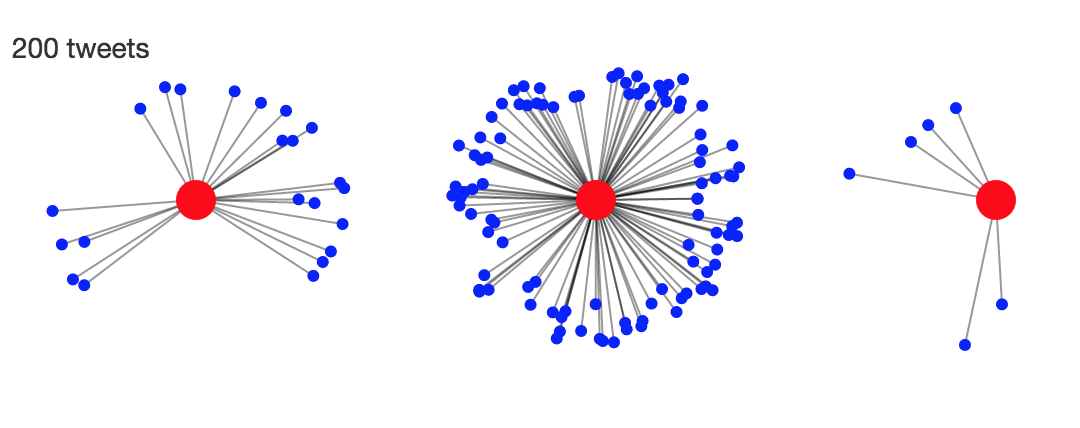
\includegraphics[width=\textwidth,height=\textheight,keepaspectratio]{src/img/clusters.png}
\caption{Example of cluster rendering\label{overflow}}
\end{figure}

{\frontend}  polls the server API at a fixed time intervals and gets the latest version of the tweets as well as their respective cluster. Using an appropriate data structure we group the tweets together based on cluster id and draw the clusters to the webpage. Drawing is done using an SVG\abbrev{SVG}{Scalable Vector Graphics} element with the help of the D3 library.
\newline
The interface presents the user a more meaningful representation of the data: tweets that belong to the same cluster are shown drawn together, also it is possible to explore the cluster and see all the messages that compose it.
\newline
The clusters will automatically update when new data comes in without the need to refresh the webpage. The application polls the API and when new messages become available it will redraw the clusters. A small optimization to the polling requests has been added: the polling interval doubles every time the request does not return with new data. This prevents the server from receiving too many requests if multiple {\frontend}  clients are running and also works similarly to the data processing step which will always take longer as more tweets are fed into the pipeline.
\newline
An explanation of Figure 3.3: We have tweets (blue dots) and centroids (the red dots). The centroid is only used as a visual cue, making it obvious which tweets belong together. Hovering over any of the blue dots to view the content of the tweet in an overlay that will appear or clicking on the red dot reveals a side menu on the right side with all the tweets that make up the cluster as well as a total.
\subsection{Deployment}
\label{deployment}
For automated deployment of the project I used Docker\footnote{https://www.docker.com}, it is an Open Source project that runs applications inside of software containers. A container is similar to a virtual machine but avoids the overhead of it by sharing the same kernel as the host. Dockerfiles are configuration files for Docker containers, they are scripts that describe the steps necessary to create the environment for the application. A Dockerfile for \project  is also available as a gist\footnote{https://gist.github.com/piatra/53c0b6d185d10eeeaf8b}. Some of the requirements of the project that the container automatically configures:
\begin{enumerate}
	\item Scala 2.10
	\item sbt 0.13.1 (Scala built tool) - Allows for task automation, running tasks and access to the Maven Central Repository for installing and updating packages 
	\item Kafka 2.9.1
	\item Java 8
	\item These are on top of Ubuntu 12.04
\end{enumerate}
The script installs the required software with appropriate versions, updates all packages and it also created all the necessary configurations. Using this setup benchmarking was greatly simplified and we were able to try out different parameters for the clustering algorithm at the same time and observe how that affected the clustering performance and quality.
Much of the testing involved in the development of the application was done on DigitalOcean. They are a PaaS\footnote{Platform as a Service} that offer virtual private servers, and one of the most useful feature they provide is the ability to start up several machines at the same time capable of running the project, each with custom performance capabilities. The servers used were equipped with 4 CPUs Intel(R) Xeon(R) CPUs and 8GB of RAM. Using virtual machines was an ideal setup for benchmarking because even though we used several different instances we were able to use the same snapshot across all machines thus ensuring a uniform testing environment. Once a container is started it will automatically begin fetching new data from Twitter and after an initial waiting period (in which the queue fills up with messages) the processing pipeline starts as well.
\newline

\section{Testing and Evaluation}
\label{sec:testing}

One of the advantages provided by the Scala programming language is its ease of manipulating collections using functions familiar to most functional programming languages such as map, reduce, filter, fold. This was an advantage that made it a perfect choice for manipulating large collections of messages.
At the same time Scala provides \textit{parallel collections}\footnote{http://docs.scala-lang.org/overviews/parallel-collections/overview.html}. These are special collections included in the standard library that offer a high level API that facilitates parallelization. Calling the \textbf{.par} method on a regular collection such as \textbf{List}s or \textbf{Vector}s transforms it into a parallel collection and one can continue using that as a regular collection but now the transformations are done in parallel.
\newline
Below is a chart that outlines the performance improvements of using parallel collections. For the final set of data containing 1000 messages the performance improvement is of 588s (9,8 minutes). 

\resizebox {\columnwidth} {!} {
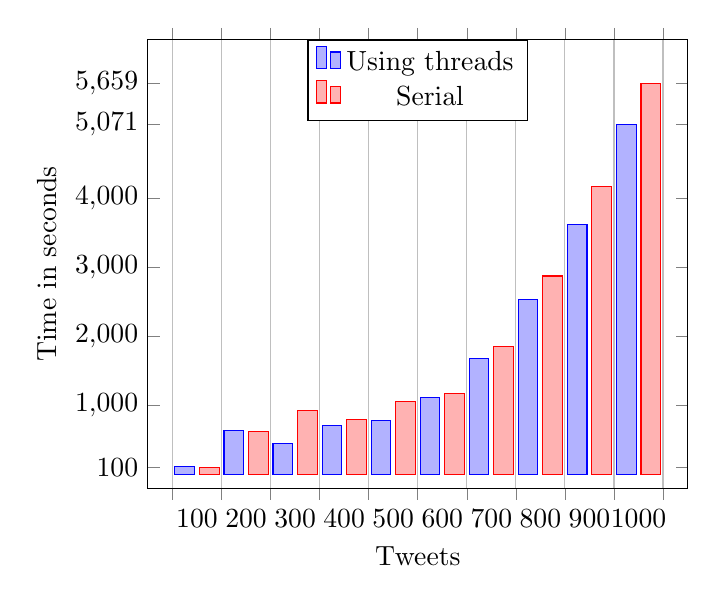
\begin{tikzpicture}
\begin{axis}[
	x tick label style={
		/pgf/number format/1000 sep=},
	ylabel= Time in seconds,
	ytick={100,1000,2000,3000,4000,5071,5659},
	xlabel= Tweets,
	enlargelimits=0.05,
	legend style={at={(0.5,1),anchor=north east},
	anchor=north},
	ybar interval=0.8,
]
\addplot 
	coordinates {(100,114) (200,637)
		 (300,445) (400,714) (500,782) (600,1116) (700,1680)
		 (800,2527) (900,3624) (1000,5071) (1100,6000)};
\addplot 
	coordinates {(100,97) (200,625)
		 (300,924) (400,791) (500,1056) (600,1178) (700,1857)
		 (800,2874) (900,4175) (1000,5659) (1100,6000)};
\legend{Using threads,Serial}
\end{axis}
\end{tikzpicture}
}

As mentioned in the \textbf{Implementation} section, each cluster generated by the K-Means algorithm has a different weight and running the algorithm multiple times can yield better results, at the cost of running time.

\resizebox {\columnwidth} {!} {
{\scalefont{0.5}
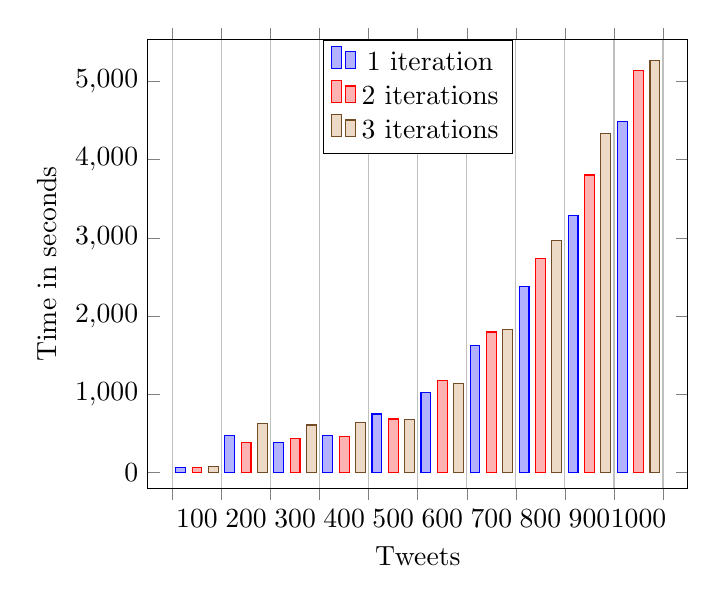
\begin{tikzpicture}
\begin{axis}[
	x tick label style={
		/pgf/number format/1000 sep=},
	ylabel= Time in seconds,
	xlabel= Tweets,
	enlargelimits=0.05,
	legend style={at={(0.5,1),anchor=north east},
	anchor=north},
	ybar interval=0.6,
]
\addplot 
	coordinates {(100,70) (200,471)
		 (300,390) (400,474) (500,749) (600,1026) (700,1626)
		 (800,2380) (900,3285) (1000,4486) (1100,5000)};
\addplot 
	coordinates {(100,63) (200,386)
		 (300,435) (400,461) (500,685) (600,1180) (700,1797)
		 (800,2733) (900,3803) (1000,5133) (1100,5000)};
\addplot
	coordinates {(100,73) (200,623)
		 (300,608) (400,638) (500,680) (600,1141) (700,1834)
		 (800,2969) (900,4330) (1000,5271) (1100,5000)};
\legend{1 iteration,2 iterations,3 iterations}
\end{axis}
\end{tikzpicture}
}
}

Above we can see how running 1, 2 or 3 iterations impacts the running time.
\newline
An advantage of using queues means that the consumer and producer processes that interact with the queue are completely decoupled. Therefore we are able to spin up several producers and consumers at the same time. Producers could either be Twitter API producers that provide the tweets, this would speed up the cold start of the application, currently it waits for 6 minutes for the queue to fill up with messages. Another producer in the pipeline is the parser that handles part-of-speech tagging and filtering of messages, this consumes raw tweets and produces tokenized messages that are stored in another queue.
\newline
Types in Scala are another optimization that yielded improved performance. Parallel collections offer improved running time by delegating the work to several threads but using incorrect types can yield unfavorable results. \textbf{List}s in Scala are collections optimized for LIFO (last-in-first-out) type of access. Although random access is possible it comes with a performance loss. This disadvantage is also present when converting to a parallel collection \textit{ParVector}, the overhead comes from the fact that all sequential collections such as lists have to be copied over to each thread. Using a different data structure improves performance especially when the quantity of messages increases.

\resizebox {\columnwidth} {!} {
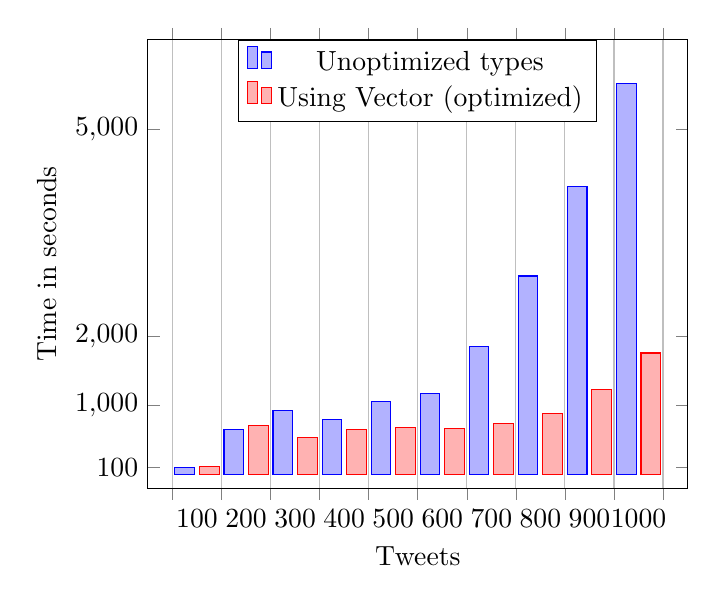
\begin{tikzpicture}
\begin{axis}[
	x tick label style={
		/pgf/number format/1000 sep=},
	ylabel= Time in seconds,
	ytick={100,1000,2000,5000},
	xlabel= Tweets,
	enlargelimits=0.05,
	legend style={at={(0.5,1),anchor=north east},
	anchor=north},
	ybar interval=0.8,
]
\addplot 
	coordinates {(100,97) (200,656)
		 (300,924) (400,791) (500,1056) (600,1178) (700,1857)
		 (800,2874) (900,4175) (1000,5659) (1100,6000)};
\addplot 
	coordinates {(100,114) (200,707)
		 (300,540) (400,646) (500,679) (600,669) (700,735)
		 (800,883) (900,1228) (1000,1758) (1100,6000)};
\legend{Unoptimized types,Using Vector (optimized)}
\end{axis}
\end{tikzpicture}
}

From the chart above we can notice a 3x speed improvement when choosing the appropriate data structures.
